\subsection{Experimentación}

En la siguiente aparatado intentaremos validar dos hipótesis: que el modelo generado realmente puede ser identificado como un hablante extranjero y al mismo tiempo que este posee un grado de inteligibilidad aceptable.

Para eso se condujo una encuesta perceptual donde, dado un participante, se le presentó un audio con una oración semánticamente impredecible, fonéticamente balanceada y con distintos grados de mezcla de español e ingles, se le pidió que la transcribiera y que intentara identificar la nacionalidad del mismo.

Para la experimentación, se generaron diez oraciones distintas variando el nivel de mezcla de los modelos generados entre $30\%$ de ingles - $70\%$ castellano hasta $70\%$ de ingles - $30\%$ de castellano.

La encuesta se realizó a través de internet, con el mismo set de instrucciones para todos los participantes y pidiendo como requerimiento la utilización de auriculares. Cada participante podía contestar como máximo 5 veces a la encuesta (otorgandoseles audios siempre distintos).

La misma se llevó a cavo desde el 18 de octubre de 2017 hasta el primero de diciembre.

\subsubsection{Interface}

A continuación se presentará la interface que utilizamos para realizar la encuesta junto con las deciciones de diseño que fueron tomadas a lo largo de la misma. 

Todos los participantes al entrar en la pagina donde se hosteaba la encuesta se encontraron con lo siguiente:

Con el objetivo de no influir el las respuestas de los participantes participantes, procuramos no darles a los participantes en ningun momento información especifica de que buscabamos con este estudio.

A cada participante se le pidió como requerimiento que realizara la encuesta con auriculares y en un lugar silencioso.

Ademas, a cada participante le pedimos que indique su genero, su edad y la provincia en la que transcurrido la mayor parte de su infancia.

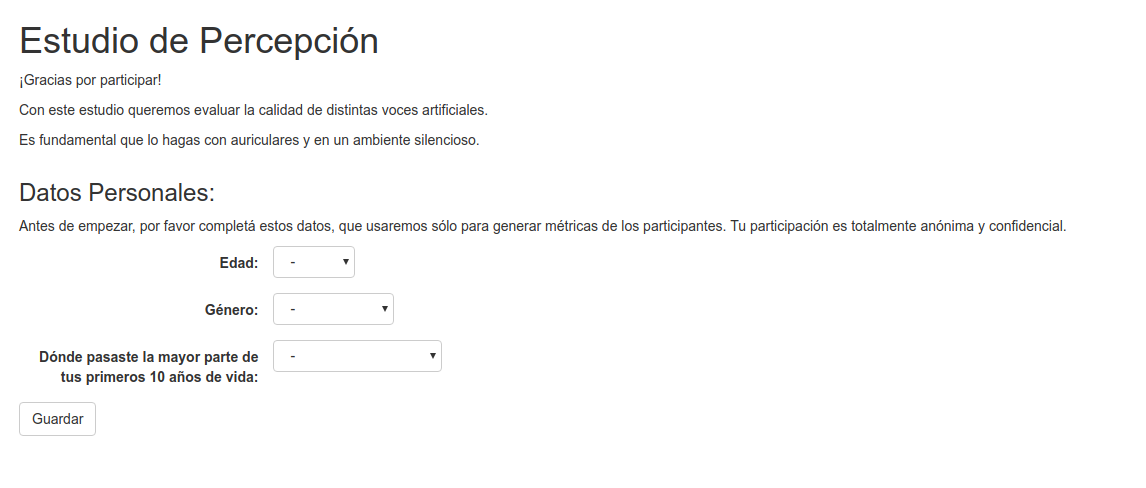
\includegraphics[scale=0.5]{estudio_online/estudio1.png}

Una vez que completaban esta información, y presionavan el boton de guardar, se les presentaba otra vista donde se le brindaban las instucciones necesarias para completar la encuesta:

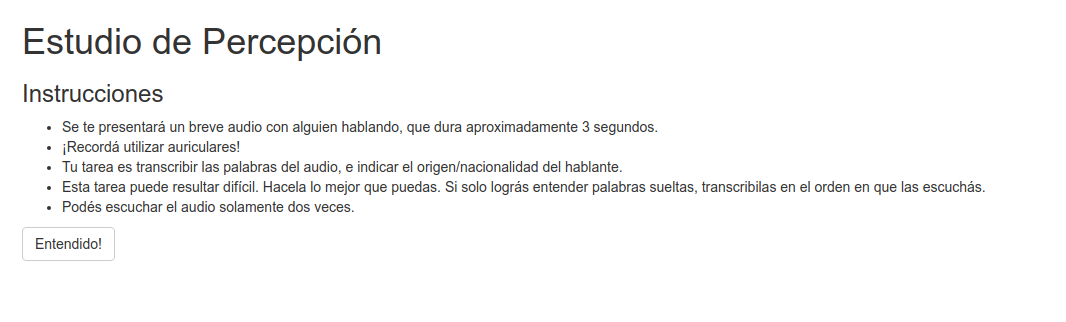
\includegraphics[scale=0.5]{estudio_online/estudio2.png}

Una vez que precionan el boton de ``entendido!'' les es presentado un audio, que pueden escuchar un maximo de 2 veces, una caja de texto libre donde escribir lo que interpretaron del mismo y una caja de texto libre donde escribir la nacionalidad que concideran es el hablante.

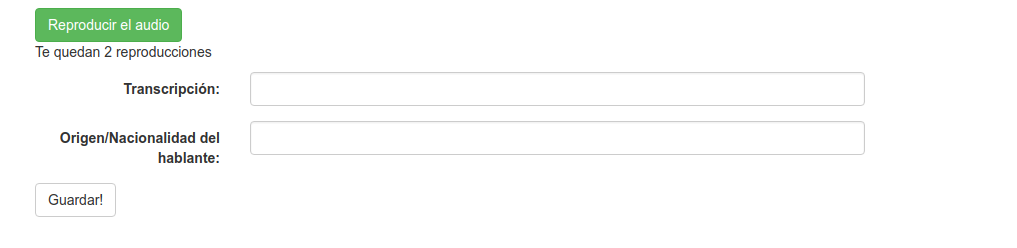
\includegraphics[scale=0.5]{estudio_online/estudio3.png}


Las oraciones presentadas fueron:

\begin{enumerate}
\item Mi montaña aguileña recorrió la esquina
\item Aquel fuerte vidrio prefirió aquel botón
\item Este enjoyado juez comprará nuestro corchete
\item Tu estrecho posavasos gritó la fechoría
\item Nuestro nublado tigre concluyó a este chupetin
\item Su profundo riñón apoyó a Julio
\item El frío churrasco oyó lo de polonia
\item Las acongojadas cotorras sonrieron a mi círculo
\item Ese gruñón perro prometió a esos cuñados
\item El nudillo Argentino perdió su vaso
\end{enumerate}


\subsection{Resultados}

Para el analisis de resultados partiremos realizando una introducción donde mostremos la demografía de los participantes. Luego un analisis mas exaustivo de la inteligibilidad y otro de la nacionalidad atribuida a la voz generada. Por ultimo intentaremos analizar ambos ejes juntos para intentar determinar el mejor grado de ingles/inteligibilidad.

\subsubsection{Datos demograficos}

Se encuestaron $109$ participantes, con los que se obtuvieron $352$ resultados.

A continuación presentaremos los datos demograficos de los participantes:

\begin{figure}[htp]
\begin{center}
$
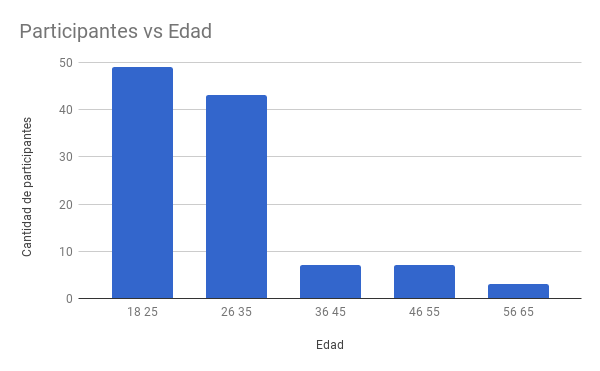
\includegraphics[scale=0.3]{datosDemograficos/edad.png}
$
\end{center}
\caption{Figure caption}
\label{pics:blablabla}
\end{figure}


En cuanto al genero de los participantes, 187 respuestas fueron brindadas por participantes del genero femenino mientras que 163 respuestas fueron respondidas por personas del genero masculino, una persona no contesto a esta pregunta.


\begin{figure}[htp]
\begin{center}
$
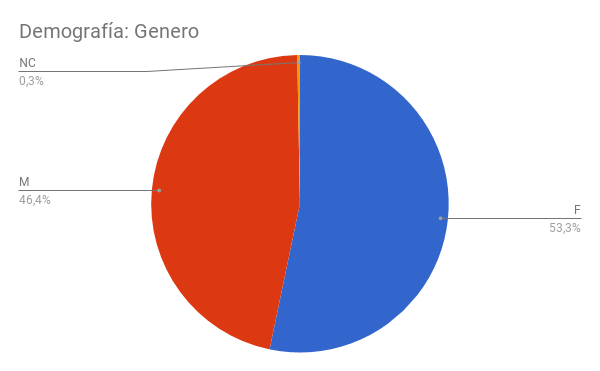
\includegraphics[scale=0.3]{datosDemograficos/genero.png}
$
\end{center}
\caption{Figure caption}
\label{pics:blablabla}
\end{figure}


Así mismo, la distribución de el lugar donde los participantes pasaron su infancia se puede ver en este grafico:


\begin{figure}[htp]
\begin{center}
$
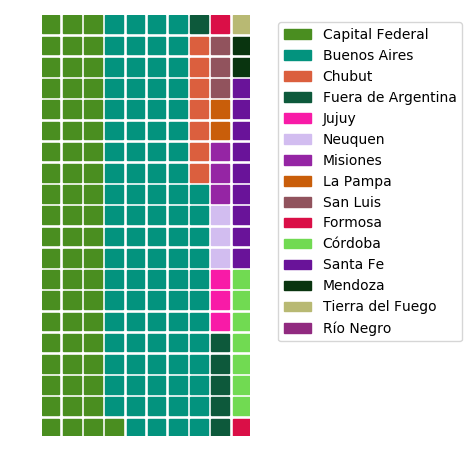
\includegraphics[scale=0.3]{datosDemograficos/infancia.png}
$
\end{center}
\caption{Figure caption}
\label{pics:blablabla}
\end{figure}

\subsubsection{Inteligibilidad}

Para el analisis de resultados utilizaremos la distancia de Levenshtein con inserciones, remociones y reemplazos. Respetando los acentos pero sin tener en cuenta mayusculas o minusculas.

Presentamos aquí los resultados obtenidos sin ningun tipo de modificación:

\begin{figure}[htp]
\begin{center}$
\begin{array}{lll}
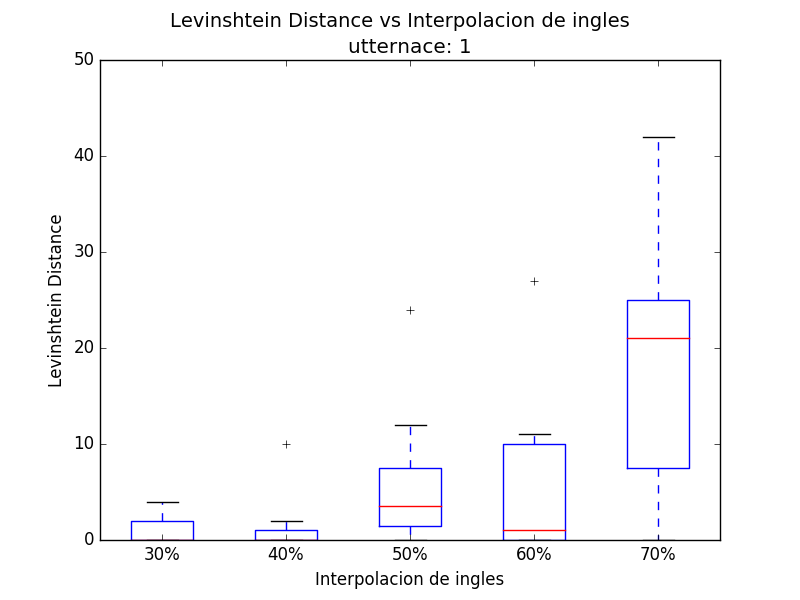
\includegraphics[width=.5\textwidth]{imagenes/plots_raw/1.png}&
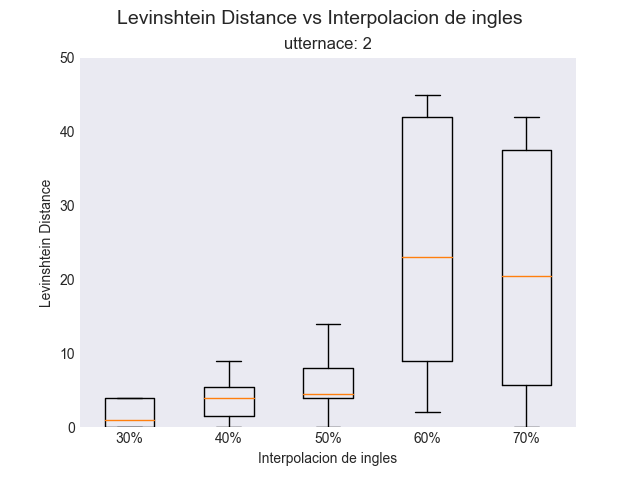
\includegraphics[width=.5\textwidth]{imagenes/plots_raw/2.png}
\end{array}$
\end{center}
\caption{Utternace 1 y 2}
\label{pics:blablabla}
\end{figure}

\clearpage

Como puede verse en la mayoría de los utternaces se puede observar que hasta el $50\%$ de mezcla castellano-ingles, se conserva el un buen grado de inteligibilidad, rondando la distancia de Levenshtein al rededor de $10$ a $20$ caracteres. Pasados el $60\%$ de ingles, se observa una disminución bruzca en la inteligibilidad, llegando a una distancia de 45 caracteres.

\begin{figure}[htp]
\begin{center}$
\begin{array}{lll}
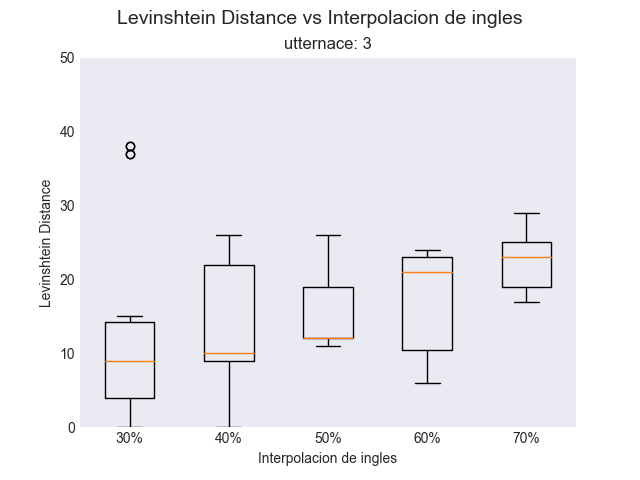
\includegraphics[width=.5\textwidth]{imagenes/plots_raw/3.png}&
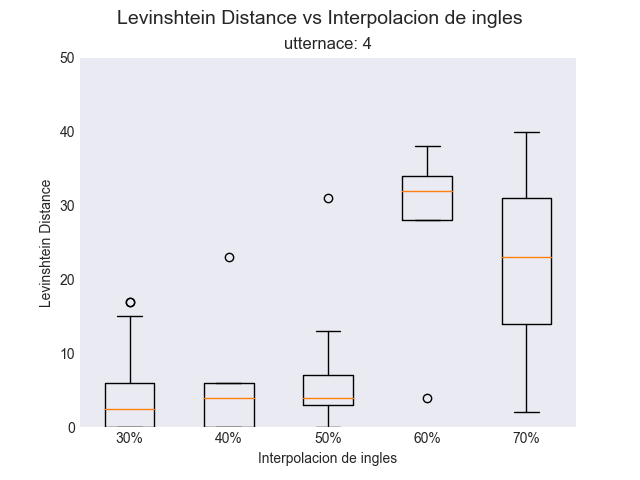
\includegraphics[width=.5\textwidth]{imagenes/plots_raw/4.png}
\end{array}$
\end{center}
\caption{Utternace 3 y 4}
\label{pics:blablabla}
\end{figure}

Analizando mas detenidamente los datos obtenidos pudimos observar algunas fallas sistematicas que podrían generar ruido en el analisis, tales como:

\begin{itemize}
	\item Los participantes escribieron de manera diferente cuando no entendieron un segmento del audio.
		\begin{itemize}
		\item Muchos de ellos escribieron: ``...'', ``....'' o simplemente omitían la palabra.
		\item En casos menos comunes: ``***'', ``???'', ``blablabla''.
		\end{itemize}
	\item En casos donde no comprendieron ninguna palabra del audio escribieron cosas como ``no entendi nada'', ``nada'', dejaron el campo vacío, etc.
	%\item Faltas ortografias del estilo: "grunion" en vez de "gruñón" que podría deberse a un teclado
	\item Utilización de signos de puntuación en las oraciones:
		\begin{itemize}
		\item Puntos finales para expresar el final de la oración o expresiones como ``(?)''.
		\item En un caso extremo, un participante el participante transcribió `` ``tu estrecho posavasos'', grito la fechoría'', cuando el utternace original solo decía ``tu estrecho portavasos gritó la fechoría''.
		\end{itemize}
	\item Omición de acentos en palabras que no resultaban ambiguas.
\end{itemize}

\begin{figure}[htp]
\begin{center}$
\begin{array}{lll}
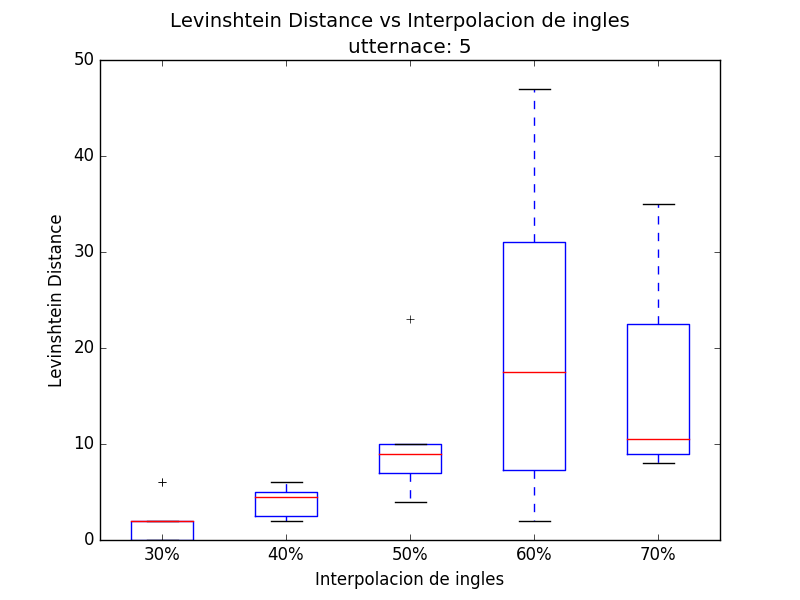
\includegraphics[width=.5\textwidth]{imagenes/plots_raw/5.png}&
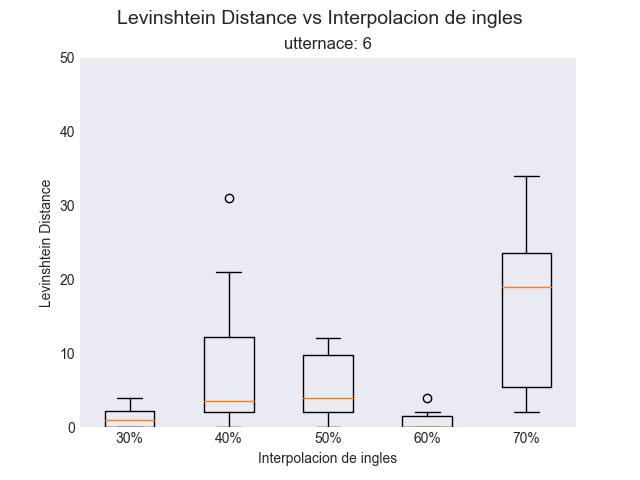
\includegraphics[width=.5\textwidth]{imagenes/plots_raw/6.png}
\end{array}$
\end{center}

\caption{Utternace 5 y 6}
\label{pics:blablabla}
\end{figure}

\begin{figure}[htp]
\begin{center}$
\begin{array}{lll}
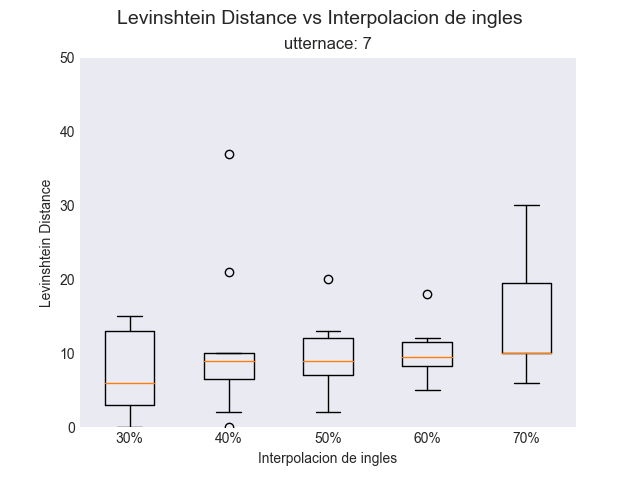
\includegraphics[width=.5\textwidth]{imagenes/plots_raw/7.png}&
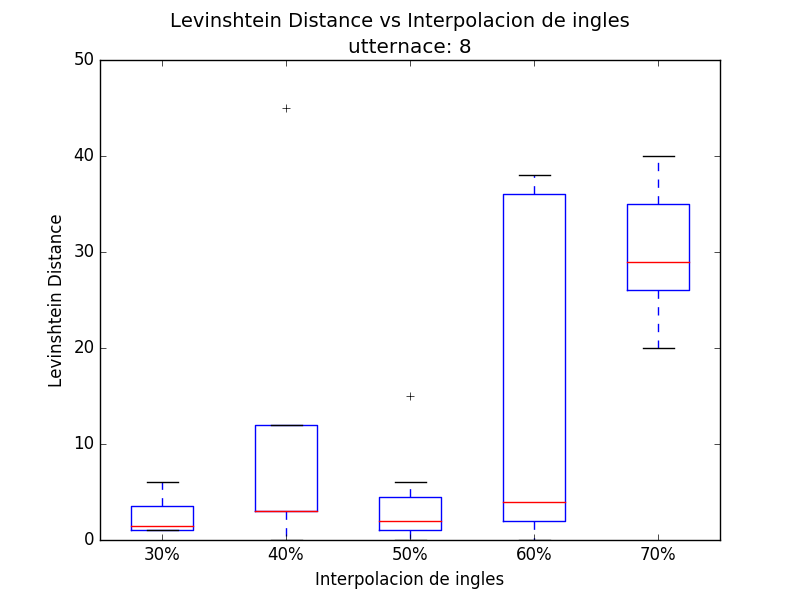
\includegraphics[width=.5\textwidth]{imagenes/plots_raw/8.png}
\end{array}$
\end{center}
\caption{Utternace 7 y 8}
\label{pics:blablabla}
\end{figure}

Para tener datos mas precisos, decidimos realizar una limpieza de los datos donde concideramos que no era disruptiva.

Los cambios fueron:

\begin{itemize}
\item corregir ``ni'' por ``ñ '' en la palabra grunion.
\item Remoción de todos los signos de puntuación. 
\item Remoción de expresiones como ``blabla'' o cualquier otra que exprese ininteligibilidad de una palabra u oración.
\item Correción de acentos en palabras no ambiguas: ``botón'', ``prefirió'', ``recorrió'', ``chupetín'', ``riñón'', ``grúñón''.
\item Las palabras que presentan ambibalencia, como : ``concluyó'' no fueron modificadas ya que concluyó/concluyo son validas.
%otros ejemplos: apoyo, enfrío
\end{itemize}
\begin{figure}[htp]
\begin{center}$
\begin{array}{lll}
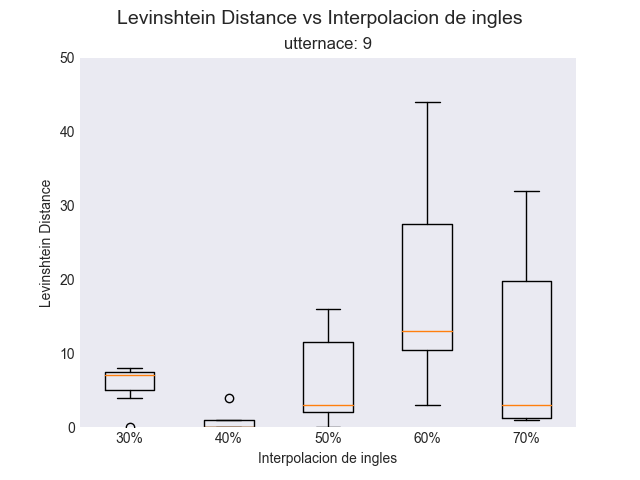
\includegraphics[width=.5\textwidth]{imagenes/plots_raw/9.png}\quad
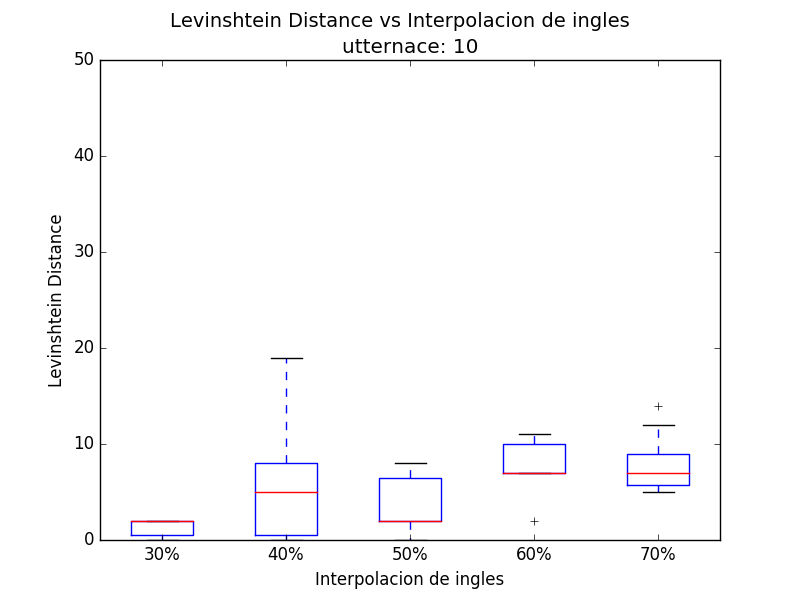
\includegraphics[width=.5\textwidth]{imagenes/plots_raw/10.png}
\end{array}$
\end{center}
\caption{Utternace 9 y 10}
\label{pics:blablabla}
\end{figure}

\clearpage
Habiendo realizado estas correcciones, ahora las distancias de Levinshtein se ven así: 

\begin{figure}[htp]
\begin{center}$
\begin{array}{lll}
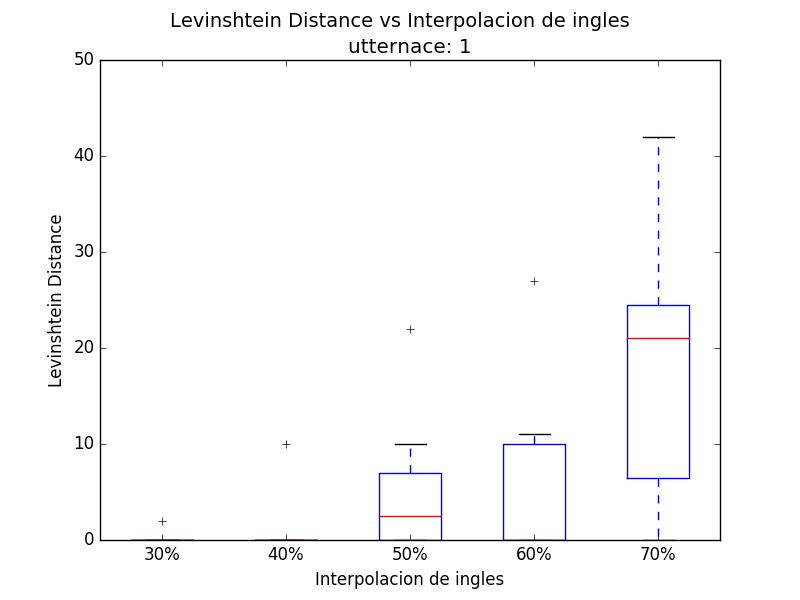
\includegraphics[width=.5\textwidth]{imagenes/plots_normalized/1.png}&
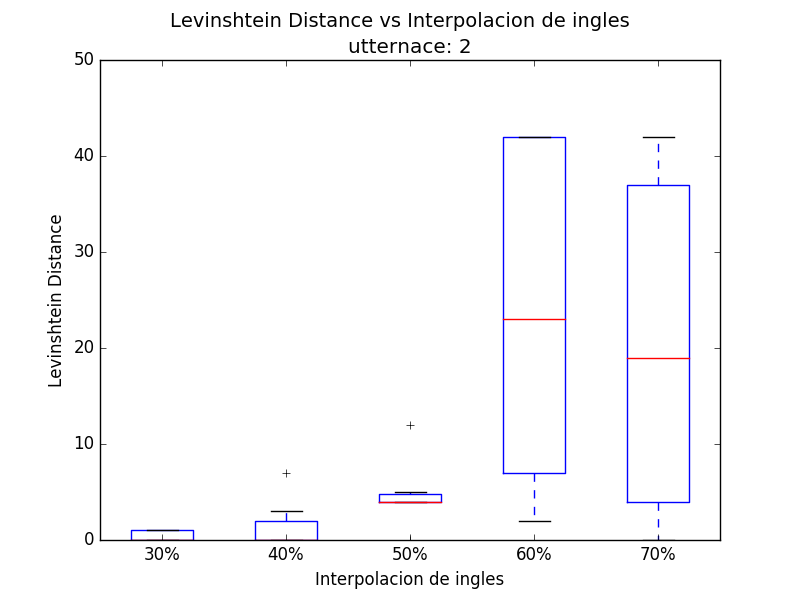
\includegraphics[width=.5\textwidth]{imagenes/plots_normalized/2.png}
\end{array}$
\end{center}
\caption{Utternace 1 y 2 Normalizados}
\label{pics:blablabla}
\end{figure}

\begin{figure}[htp]
\begin{center}$
\begin{array}{lll}
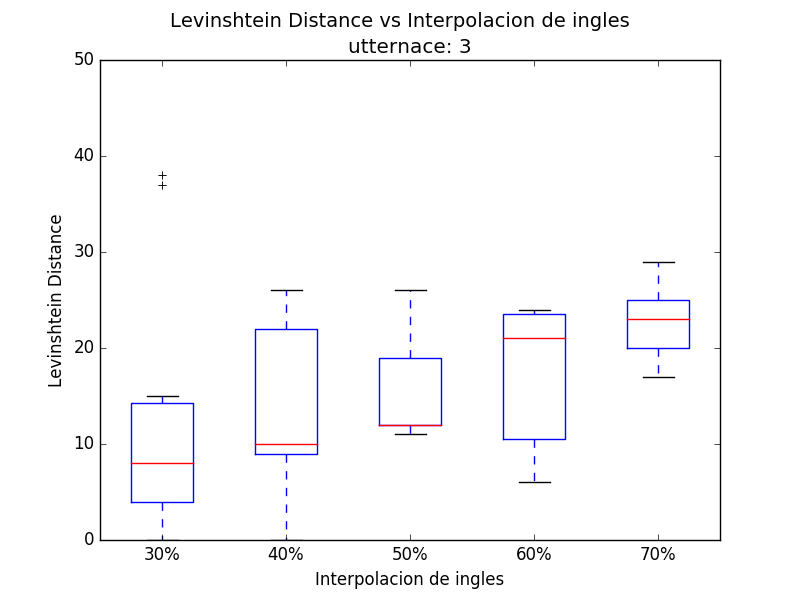
\includegraphics[width=.5\textwidth]{imagenes/plots_normalized/3.png}&
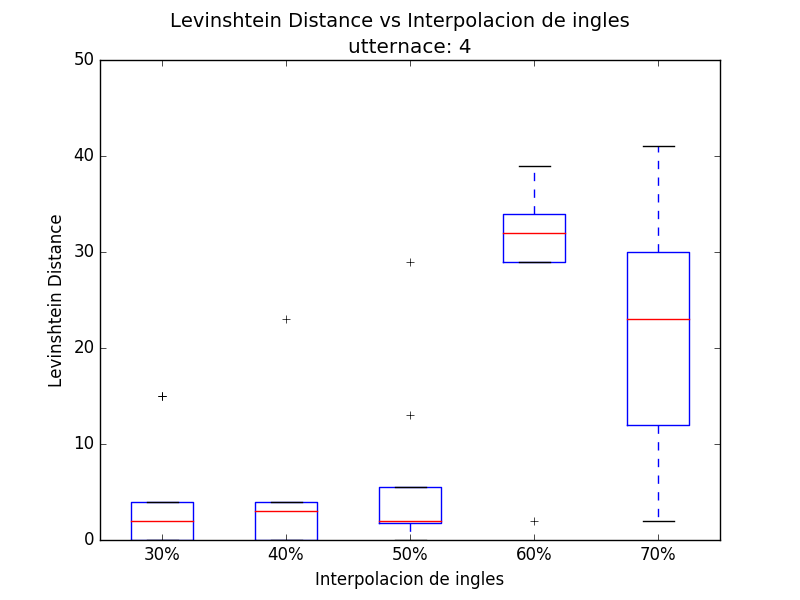
\includegraphics[width=.5\textwidth]{imagenes/plots_normalized/4.png}
\end{array}$
\end{center}
\caption{Utternace 3 y 4 Normalizados}
\label{pics:blablabla}
\end{figure}

\begin{figure}[htp]
\begin{center}$
\begin{array}{lll}
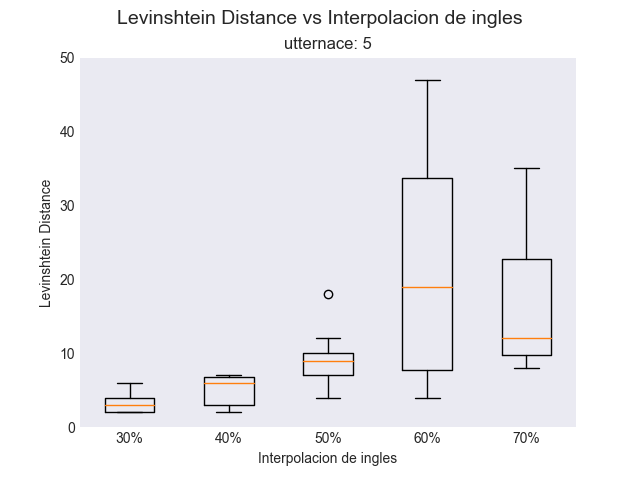
\includegraphics[width=.5\textwidth]{imagenes/plots_normalized/5.png}&
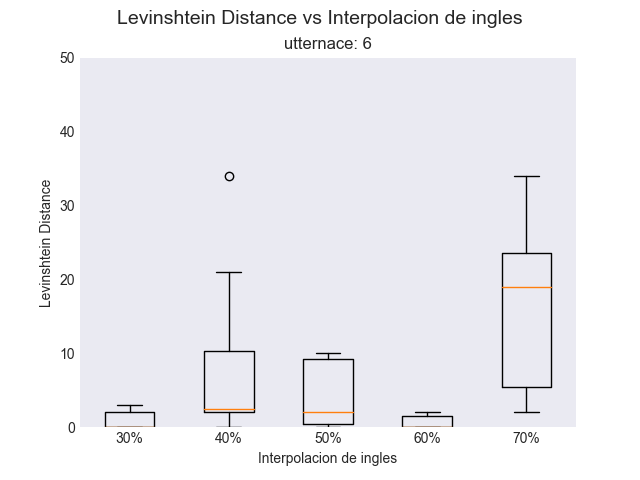
\includegraphics[width=.5\textwidth]{imagenes/plots_normalized/6.png}
\end{array}$
\end{center}

\caption{Utternace 5 y 6 Normalizados}
\label{pics:blablabla}
\end{figure}

\begin{figure}[htp]
\begin{center}$
\begin{array}{lll}
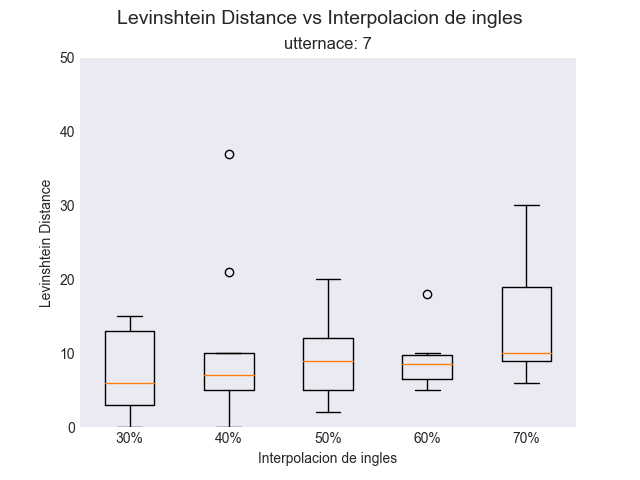
\includegraphics[width=.5\textwidth]{imagenes/plots_normalized/7.png}&
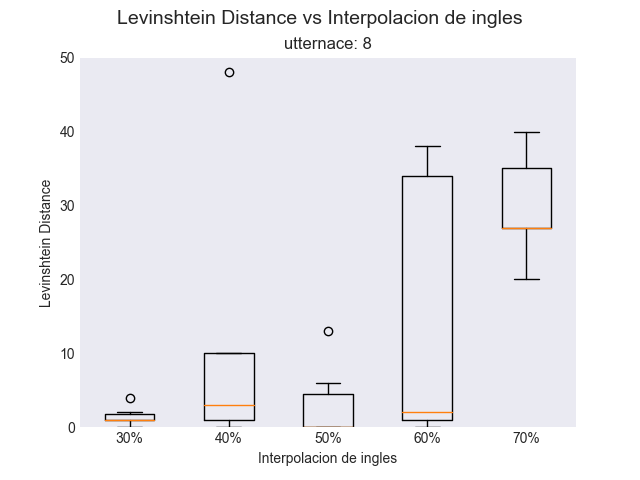
\includegraphics[width=.5\textwidth]{imagenes/plots_normalized/8.png}
\end{array}$
\end{center}

\caption{Utternace 7 y 8 Normalizados}
\label{pics:blablabla}
\end{figure}
\begin{figure}[htp]
\begin{center}$
\begin{array}{lll}
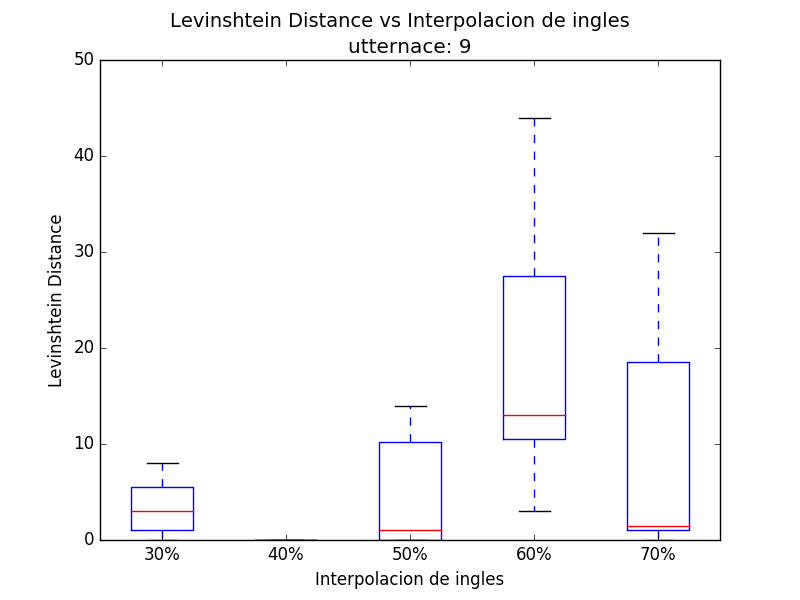
\includegraphics[width=.5\textwidth]{imagenes/plots_normalized/9.png}&
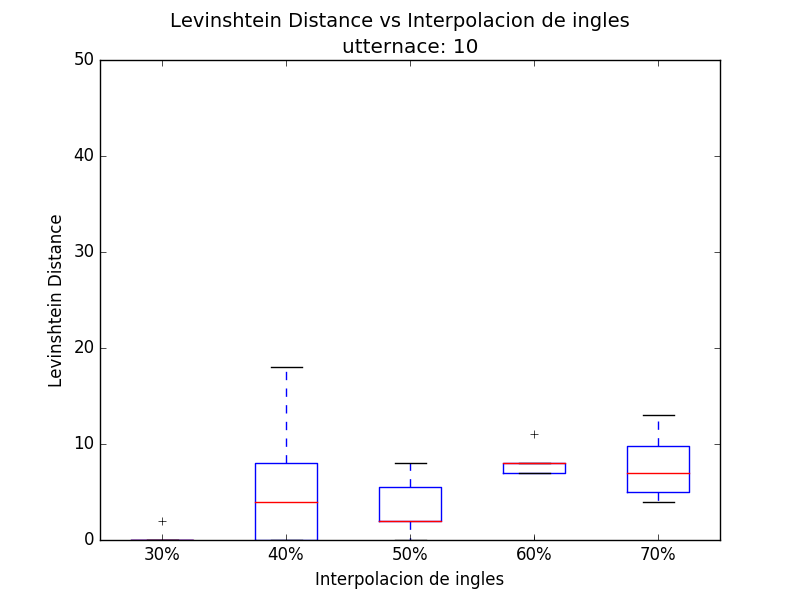
\includegraphics[width=.5\textwidth]{imagenes/plots_normalized/10.png}
\end{array}$
\end{center}
\caption{Utternace 9 y 10 Normalizados}
\label{pics:blablabla}
\end{figure}

Con esta estandaricación de los datos, trataremos de darles un peso intuitivo que nos permitan sistematizar el analisis.

Por ejemplo, tomando el utternace $8$ de las fraces utilizadas en la experimentación: 

\begin{itemize}
	\item ``Las acongojadas cotorras sonrieron a mi círculo''
\end{itemize}

Podemos observar que:

\begin{itemize}
	\item Distancia 0: ``Las acongojadas cotorras sonrieron a mi círculo''
	\item Distancia 10: ``Las acontojadas culturas sonrieron en semicírculo''
	\item Distancia 20: ``Plaza sombreada con sombrero sonrieron en mi círculo''
	\item Distancia 30: ``sonrieron en mi círculo''
	\item Distancia 40: ``círculo''
	\item Distancia 48: ``''
\end{itemize}

A partir de esto, para este trabajo vamos a tomar que una distancia de Levinshtein

\begin{itemize}
	\item Distancia 0-10: Buena Inteligibilidad
	\item Distancia 10-20: Mediana Inteligibilidad
	\item Distancia 20-40: Baja Inteligibilidad
	\item Distancia 40-: Inteligibilidad nula
\end{itemize}


Con este baseline, podemos ver que para una interpolación de ingles de $30\%$ 96 de los $106$ participantes comprendieron de manera adecuada el texto con una inteligibilidad alta. Los 10 restantes obtuvieron una inteligibilidad media. 

Para la interpolación $40\%$ ingles - $60\%$ castellano, de un total de $67$ participantes, $57$ obtuvieron una inteligibilidad alta, $2$ una inteligibilidad media, $5$ una baja y 3 una inteligibilidad nula.

Para la interpolación $50\%$ ingles - $50\%$ castellano, de un total de $75$ participantes, $57$ obtuvieron transcribir el audio demostrando una buena inteligibilidad, mientras que $14$ tuvieron una inteligibilidad media y $4$ una inteligibilidad baja.

Para todas las interpolaciones enunciadas previamente, los errores mas comunes varían desde falta de acentos en palabras como ``concluyó'' ambiguas hasta faltas de inteligibilidad en palabras con cierta complegidad como ``aguileña'' o ``gruñon''.

Para el utternace 3: ``este enjoyado juez comprará nuestro corchete'' observamos que la mayoría de los participantes cometieron errores al transcribir la palabra ``juez'' que confundieron de manera sistematica con palabras sonoramente similares como ``fue'', y ``enjoyado'' que transcribieron como ``enfollado'', ``enrollado'' y la conjugación exacta del verbo comprar.

Para los grados de interpolación $60\%$ ingles - $40\%$ castellano y $70\%$ ingles - $30\%$ castellano, se pueden observar un aumento notable de la variabilidad en las respuestas. Para el primero, de las $70$ respuestas obtenidas, $40$ participantes lograron transcribir con un buen grado de inteligibilidad los audios, $6$ obtuvieron una inteligibilidad media, y $24$ transcribieron el audio con una inteligibilidad baja o nula.

Para $70\%$ ingles - $30\%$ castellano, la diferencia es todavía mas marcada, de los $68$ resultados obtenidos, $28$ obtuvieron lograron transcribir el audio con un buen grado de inteligibilidad, $8$ con un grado medio y $32$ con un grado bajo o nulo de inteligibilidad.

Consideramos estos resultados tan dispares pueden deberse a dos motivos:

El primero, caracteristicas particulares de los participantes y sus capacidades para dicernir palabras incluso cuando presentan defectos en la pronunciación del hablante. En particular, el utternace $4$ muestra como para un mismo audio, con caracteristicas similares $2$ participantes de los 9 que realizaron la transcripción, obtuvieron distancias $2$ y $6$ en sus transcripciones.

El segundo motivo puede deberse a caracteristicas particulares de los utternaces o del modelo utilizado para generar la voz: el utternace $10$, donde el $6$ de los $8$ participantes obtuvieron una buena transcripcion del audio, y el utternace $8$, donde todos los participantes transcribieron el audio con inteligibildiad baja o nula, parecen demostrar esto. O bien la dificultad de los utternaces es variable o, lo que es todavía mas probable, llegado cierto punto en la interpolación, algunos fonemas empiezan a ``romperse'' o se alejan demasiado del fonema castellano correcto y terminan por disminuir la claridad de la voz.


%Agregar:
% python levinshteinFor.py 0
% Alta int: 96
% Media int: 10
% Baja int: 0
% nula: 4
% python levinshteinFor.py 1
% Alta int: 57
% Media int: 2
% Baja int: 5
% nula: 3
% porque nula? ver esto
\recordar
% python levinshteinFor.py 2
% Alta int: 57
% Media int: 14
% Baja int: 4
% nula: 0
% python levinshteinFor.py 3
% Alta int: 40
% Media int: 6
% Baja int: 11
% nula: 13
% python levinshteinFor.py 4
% Alta int: 28
% Media int: 8
% Baja int: 20
% nula: 12


\clearpage
\subsection{Analisis de Nacionalidad}


En esta sección analizaremos los resultados de las nacionalidades que los participantes atribuyeron a la voz.

Dado que en esta instancia se le le permitió a los participantes ingresar texto libre las respuestas resultaron bastante heterogeneas. Los participantes tomaron la consigna de manera diferente, pudiendo encontrarse respuestas que no pueden ser atribuidos exactamente a una nacionalidad. Ejemplo de alguas respuestas: Latino, Anglo, Robot, España (sur).

Concideramos que las respuestas de la indole ``robot'', ``es una voz artificial'', no son validas ya que no aportan información para esta investigación.

Por esta razón, en esta instancia decidimos agrupar las respuestas en cuatro grupos logicos:

\begin{itemize}
	\item Hispanohablante: Latino, Argentino, Español, Uruguayo, Centroamericano, Boliviano, Mexicano, Colombiano
	\item Angloparlante: Estadounidense, Ingles, Irlandes, Canadiense, Anglo
	\item No sabe/No contesta: Robot, no se
	\item Otro: Ruso, Brasiltiño
\end{itemize}

Con estas agrupaciones, presentamos las nacionalidades atribuidas a la voz generada para cada punto de la interpolación.

\begin{figure}[htp]
\begin{center}$
\begin{array}{lll}
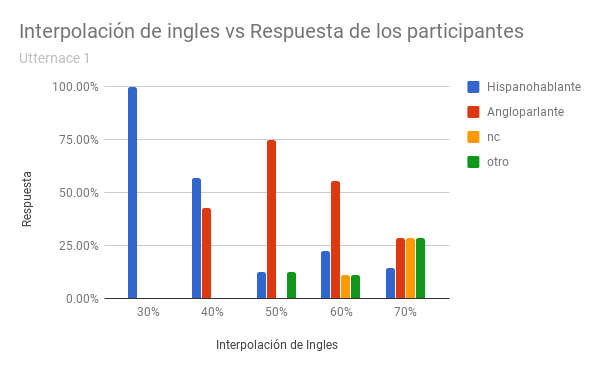
\includegraphics[width=.5\textwidth]{imagenes/nacionalidades/1.png}&
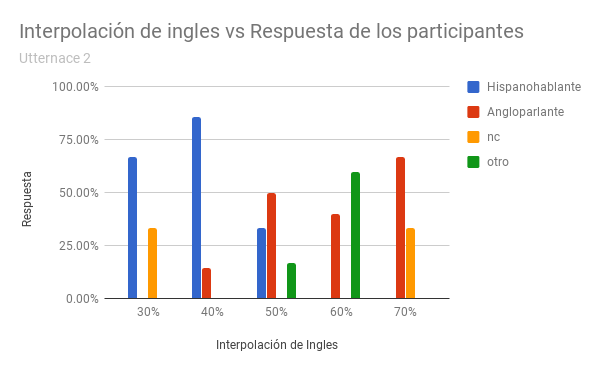
\includegraphics[width=.5\textwidth]{imagenes/nacionalidades/2.png}
\end{array}$
\end{center}
\caption{Utternace 1 y 2}
\label{pics:blablabla}
\end{figure}

De estos resultados podemos observar que con $30\%$ de interpolación de ingles, los participantes coinciden en que la voz puede atribuirse a una persona de habla nativa española.

\begin{figure}[htp]
\begin{center}$
\begin{array}{lll}
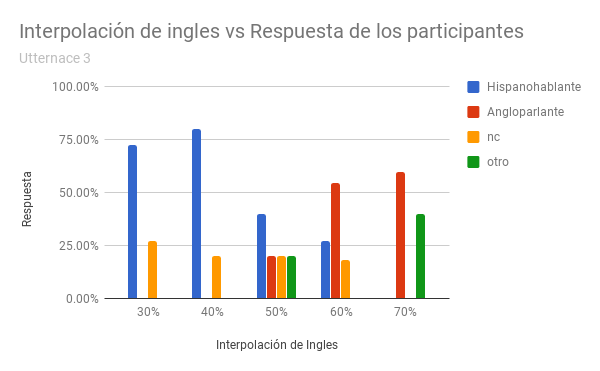
\includegraphics[width=.5\textwidth]{imagenes/nacionalidades/3.png}&
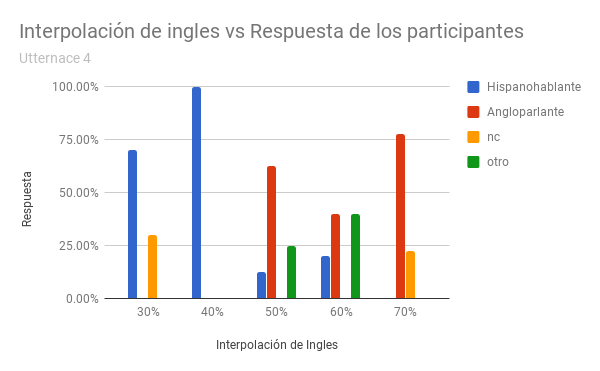
\includegraphics[width=.5\textwidth]{imagenes/nacionalidades/4.png}
\end{array}$
\end{center}
\caption{Utternace 3 y 4}
\label{pics:blablabla}
\end{figure}

Para una mezcla de $40\%$ ingles, puede verse que no hay una decición concluyente con respecto a la nacionalidad del hablante. Por ejemplo en el utternace 3 el $80\%$ de los participantes coincide que la voz pertenece a un hablante de habla hispana, mientras que en el utternace 9 el $60.00\%$ de los participantes concidera que la voz pertenece a un hablante de habla anglosajona.

Esta gran disparidad de resultados entre distintos utternaces se puede atribuir a las caracteristicas particulares de cada utternace. En particular el utternace 9: ``Ese gruñón perro prometió a esos cuñados'' contiene una /r bibrante que resulta muy notoria al pronunciarse con una intensidad menor a la esperada y es atribuida, en general, a un hablante extrangero.
%perro vibrante múltiple alveolar sonora

Bajo esta supocición observamos que los otros utternaces que presentan este fonema:

\begin{itemize}
\item Utternace 1: ``Mi montaña aguileña recorrió la esquina'' 
\item Utternace 6: ``Su profundo riñón apoyó a Julio''
\item Utternace 7: ``El frío churrasco oyó lo de polonia''
\item Utternace 8: ``Las acongojadas cotorras sonrieron a mi círculo''
\end{itemize}

Tambien presentan un mayor porcentaje de atribuciones a nacionalidad anglosajona.

\begin{figure}[htp]
\begin{center}$
\begin{array}{lll}
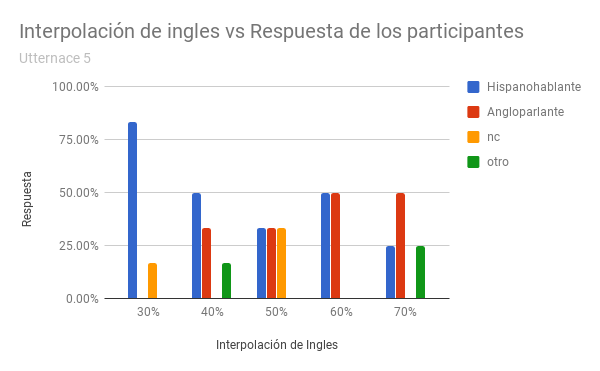
\includegraphics[width=.5\textwidth]{imagenes/nacionalidades/5.png}&
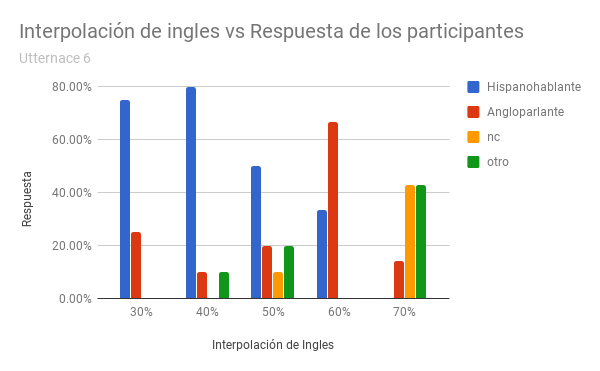
\includegraphics[width=.5\textwidth]{imagenes/nacionalidades/6.png}
\end{array}$
\end{center}
\caption{Utternace 5 y 6}
\label{pics:blablabla}
\end{figure}

Con $50\%$ y $60\%$ de ingles los resultados son similares. obtenemos que aproximadamente en el $50\%$ de los utternaces, mas de la mitad de los participantes concideraron que la voz pertenecía a un anglosajon hablando castellano. Para estos grados de interpolación tambien podemos observar que en un $80\%$ de los utternaces al menos un $20\%$ de los participantes atribuyen la nacionalidad del hablante a un no nativo no anglosajon hablando castellano.

\begin{figure}[htp]
\begin{center}$
\begin{array}{lll}
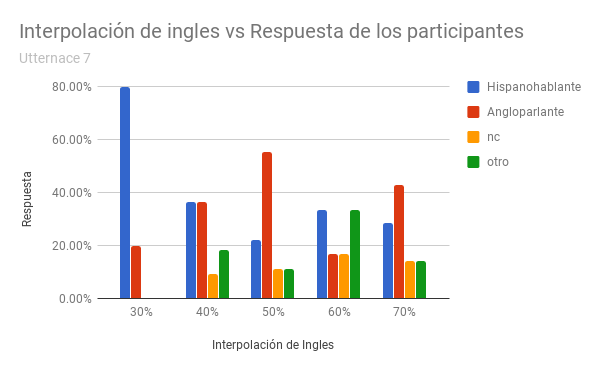
\includegraphics[width=.5\textwidth]{imagenes/nacionalidades/7.png}&
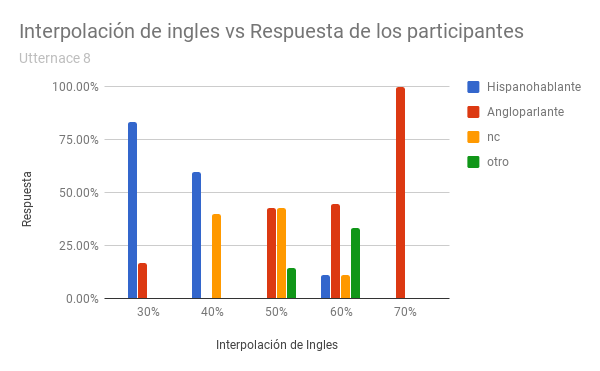
\includegraphics[width=.5\textwidth]{imagenes/nacionalidades/8.png}
\end{array}$
\end{center}
\caption{Utternace 7 y 8}
\label{pics:blablabla}
\end{figure}

Con $70\%$ de interpolación, en el $80\%$ de los utternaces se puede apreciar que al menos $50\%$ de los participantes dijo que el hablante era de origen anglosajon. Mas aún, en el $40\%$ de los utternaces el $75\%$ de los participantes coincidió que la voz era de angloparlante. Tambien podemos ver que para este grado de interpolación en el $70\%$ de los utternaces ningun participante concidera que la voz sea de habla hispana. En el $30\%$ restante, $25\%$ de los participantes o menos concideran que la voz pertenezca a un hispanohablante.

\begin{figure}[htp]
\begin{center}$
\begin{array}{lll}
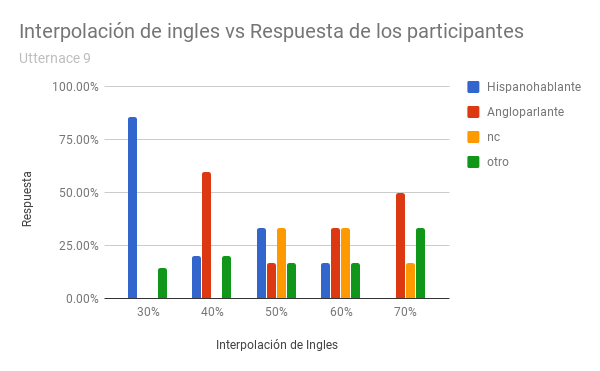
\includegraphics[width=.5\textwidth]{imagenes/nacionalidades/9.png}&
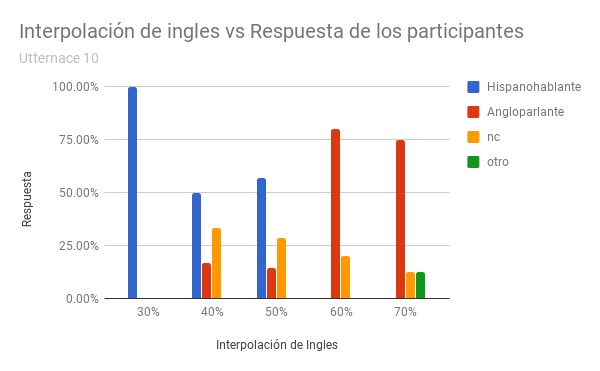
\includegraphics[width=.5\textwidth]{imagenes/nacionalidades/10.png}
\end{array}$
\end{center}
\caption{Utternace 9 y 10}
\label{pics:blablabla}
\end{figure}

%grafico general mostrando como crece el grado de ingles?

%conclucion mas general: aunque en muchos casos los participantes atribuyeron a la voz como un extrangero no anglosajon, tambien tener en cuenta que se esta intentando identificar la nacionalidad de un hablante con tan solo con una oración como referencia.

Hasta ahora analizamos los dos ejes de nuestra hipotesis por separado (por un lado, inteligibilidad, por otro, nacionalidad atribuida a la voz). En el ultimo apartado de la investigación buscaremos sacar concluciones al componer ambos ejes en un mismo analisis.

\subsection{Resultados Generales de la experimentación}

Del analisis de los graficos se desprende que dependiendo del grado inteligibilidad/probabilidad de que un participante reconozca la voz como inglesa, es posible elegir un grado diferente de interpolación ingles castellano.

Segun el experimento realizado, es posible generar una voz que sea identificada con probabilidad $0.6$ como una voz anglosajona, pero a cambio estaremos sacrificando inteligibilidad, llegando al caso donde el oyente no comprenda nada de lo que se le dijo. 

\begin{figure}[htp]
\begin{center}$
\begin{array}{lll}
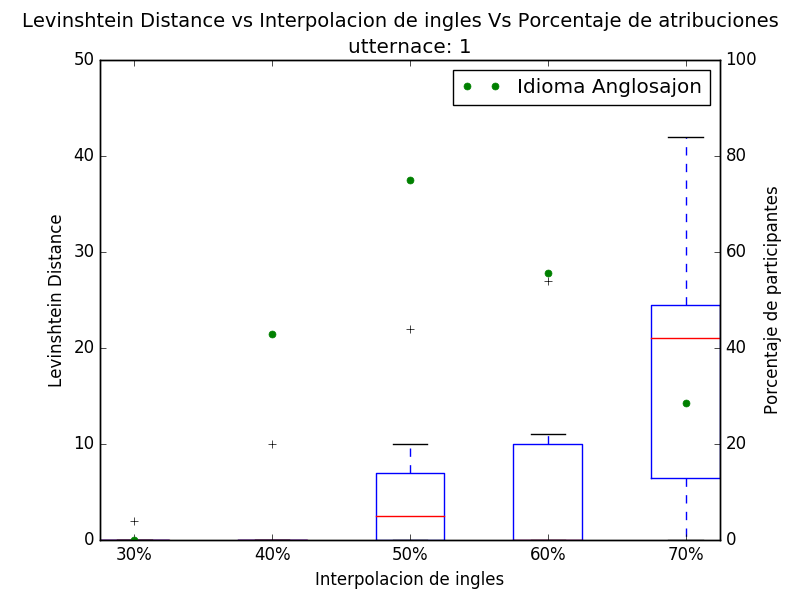
\includegraphics[width=.5\textwidth]{imagenes/nacVsPlot/1.png}&
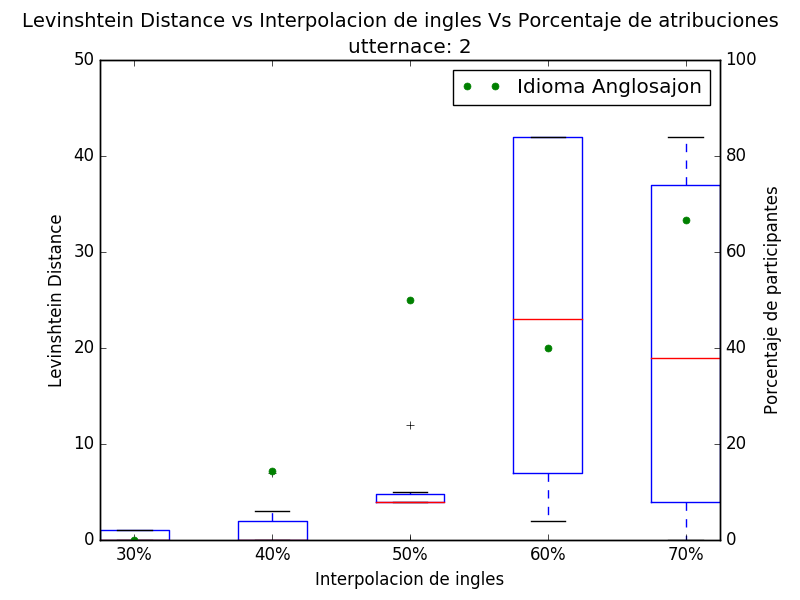
\includegraphics[width=.5\textwidth]{imagenes/nacVsPlot/2.png}
\end{array}$
\end{center}
\caption{Utternace 1 y 2}
\label{pics:blablabla}
\end{figure}

\begin{figure}[htp]
\begin{center}$
\begin{array}{lll}
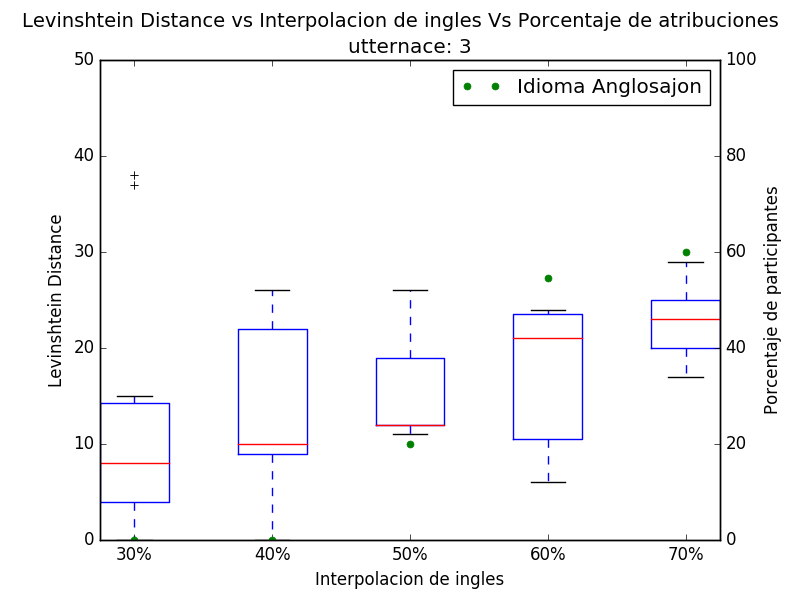
\includegraphics[width=.5\textwidth]{imagenes/nacVsPlot/3.png}&
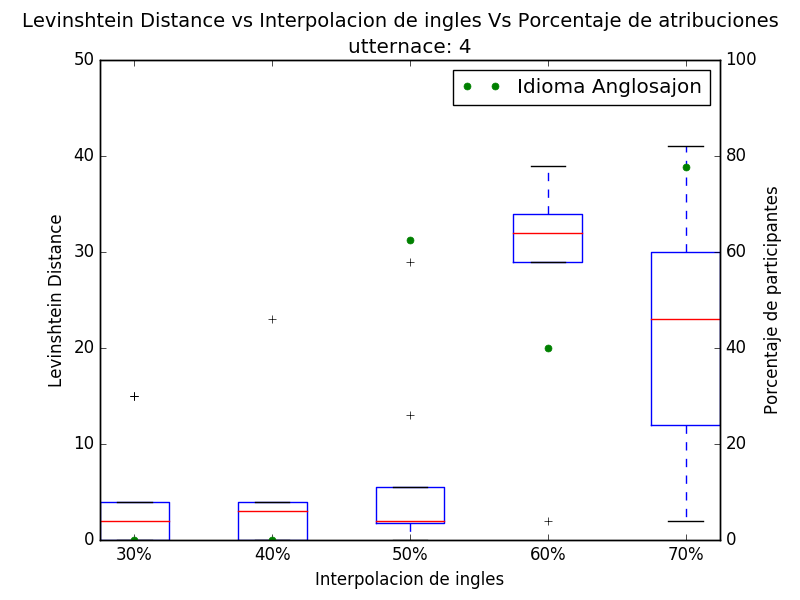
\includegraphics[width=.5\textwidth]{imagenes/nacVsPlot/4.png}
\end{array}$
\end{center}
\caption{Utternace 3 y 4}
\label{pics:blablabla}
\end{figure}

\begin{figure}[htp]
\begin{center}$
\begin{array}{lll}
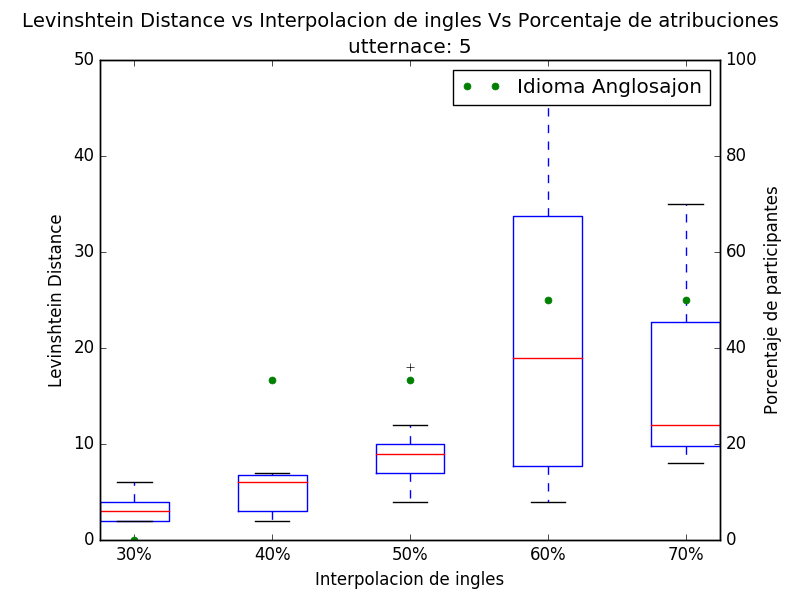
\includegraphics[width=.5\textwidth]{imagenes/nacVsPlot/5.png}&
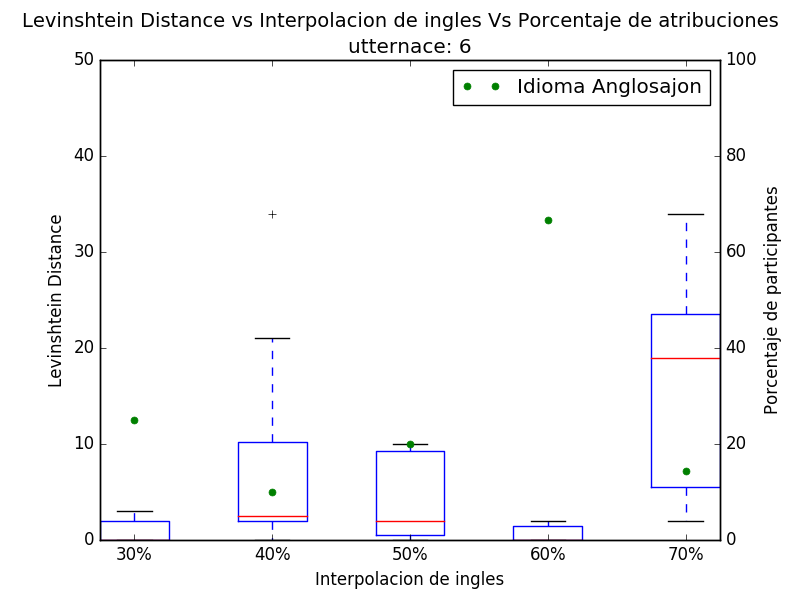
\includegraphics[width=.5\textwidth]{imagenes/nacVsPlot/6.png}
\end{array}$
\end{center}
\caption{Utternace 5 y 6}
\label{pics:blablabla}
\end{figure}

\begin{figure}[htp]
\begin{center}$
\begin{array}{lll}
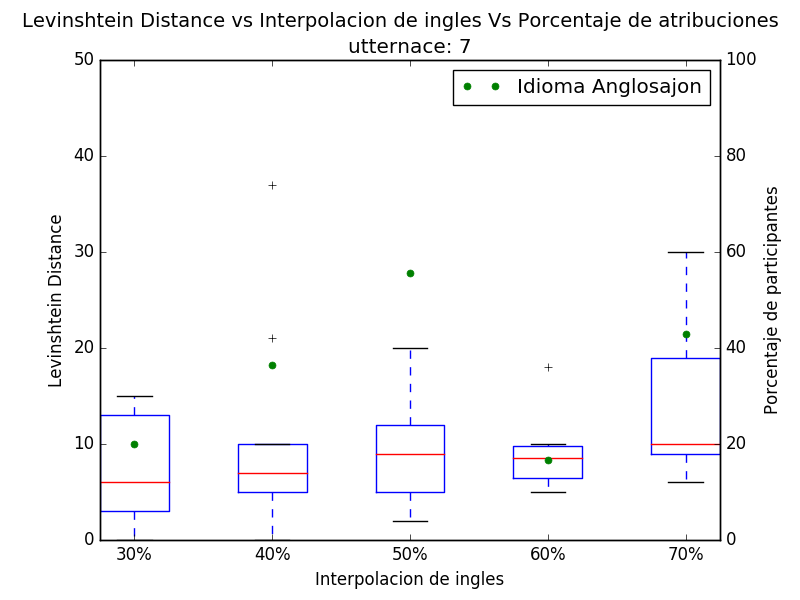
\includegraphics[width=.5\textwidth]{imagenes/nacVsPlot/7.png}&
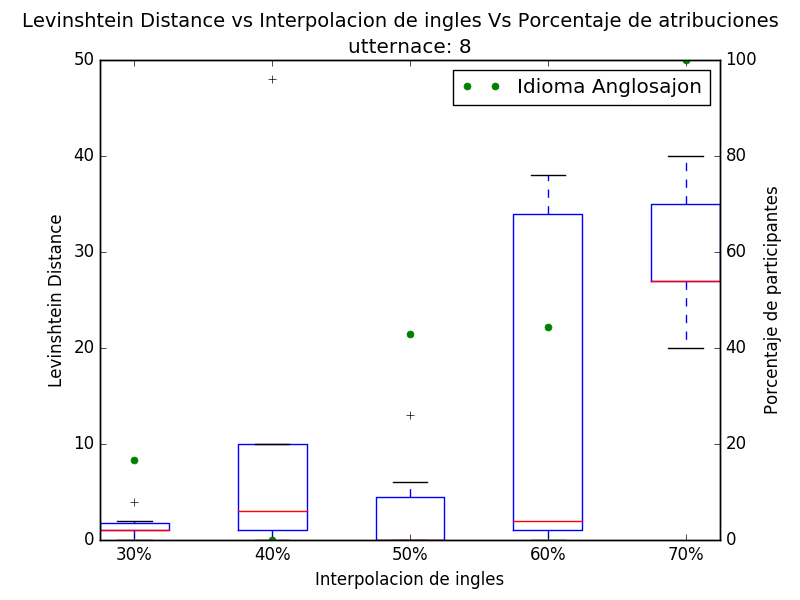
\includegraphics[width=.5\textwidth]{imagenes/nacVsPlot/8.png}
\end{array}$
\end{center}
\caption{Utternace 7 y 8}
\label{pics:blablabla}
\end{figure}

\begin{figure}[htp]
\begin{center}$
\begin{array}{lll}
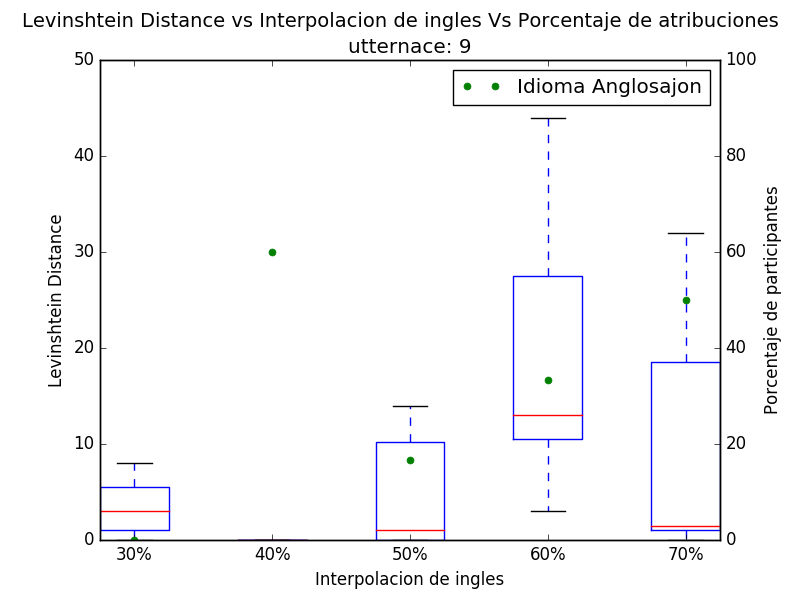
\includegraphics[width=.5\textwidth]{imagenes/nacVsPlot/9.png}&
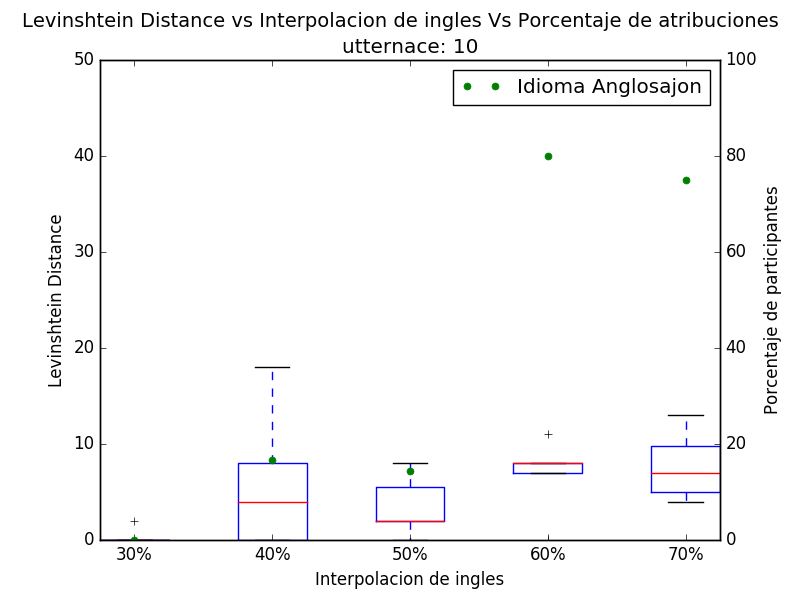
\includegraphics[width=.5\textwidth]{imagenes/nacVsPlot/10.png}
\end{array}$
\end{center}
\caption{Utternace 9 y 10}
\label{pics:blablabla}
\end{figure}




